\documentclass[conference]{IEEEtran}

\usepackage{times}
\usepackage[numbers]{natbib}
\usepackage{graphicx}
\graphicspath{{figures/}}
\usepackage{amsmath}
\usepackage{amssymb}
\usepackage{booktabs}
\usepackage{tabularx}
\usepackage{multirow}
\usepackage{xcolor}
\usepackage{caption}
\usepackage[bookmarks=true,colorlinks=true,
            linkcolor=black,urlcolor=blue,citecolor=black]{hyperref}
\usepackage{url}

\newcolumntype{C}{>{\centering\arraybackslash}X}

\begin{document}

\title{4DW-VLA: 4D Trajectory-Conditioned Mixture-of-Transformers\\
       for Multimodal Robotic Manipulation}

\author{Gang Luo\\Daohe Tongtai}

\maketitle

% ====================================================================
\begin{abstract}
Foundation vision-language-action (VLA) models have made rapid progress on
robotic manipulation, yet they still under-use the sensors a robot actually
has: most policies consume 2D images, inject little metric spatial structure,
and treat heterogeneous modalities as a single undifferentiated token stream.
We argue that effective manipulation policies should (i)~reason about the
robot's own 3D pose over time and (ii)~learn future dynamics as an
action-facing training signal, without paying video-generation cost at
deployment. We introduce \textbf{4DW-VLA}, a three-path
mixture-of-transformers policy that co-trains three complementary objectives
on a frozen vision-language backbone: future 4D keypoint trajectories
obtained from forward kinematics, future-video prediction conditioned on
those tracks, and chunked action generation. At inference the keypoint
expert is retained and continues to condition the action expert; only the
video generator is dropped, so the policy pays no video-generation cost.
On three RoboTwin~2.0 tasks after a common 76-epoch post-training schedule,
4DW-VLA matches or exceeds two recent VLA baselines across all evaluated splits, with the largest advantage
under domain randomization, consistent with the claim that
embodiment-centric 4D supervision supplies spatial structure that
image-only VLAs lack.
\end{abstract}

\IEEEpeerreviewmaketitle

% ====================================================================
\section{Introduction}
\label{sec:intro}

\IEEEPARstart{L}{earning-based} policies have shown strong performance in robotic
manipulation~\cite{rt1,rt2,chi2023diffusion,zhao2023act,kim2024openvla,black2024pi0}.
Scaling vision-language models (VLMs) into vision-language-action (VLA)
policies~\cite{rt2,kim2024openvla,black2024pi0,liu2024rdt,internvla15} has
further improved instruction following and few-shot adaptation. However, these
policies often remain brittle under novel scenes, objects, and
distractors~\cite{xie2024decomposing}, and they typically consume only RGB
images even though a robot is a multi-sensor system operating in a metric 3D
workspace.

We identify three recurring gaps. First, and most fundamentally,
\textbf{privileged, non-visual signals are fused into VLA backbones through
a single, undifferentiated attention pattern}. Whether the extra signal is a
manipulator's own joint geometry, a distilled future-dynamics code, or a
sub-task plan, most architectures give it no dedicated capacity: it is
either concatenated into the same token stream as everything else, or
bolted on as a residual branch with its own encoder and decoder. Neither
treats the signal as a first-class citizen of the backbone's own attention
computation, and neither is retained past training when the signal is
genuinely useful at deployment. Second,
\textbf{spatial information is under-used}. A manipulator's own joints
already determine metric end-effector and link poses through forward
kinematics (FK); this signal is free, temporally dense, and aligned with the
action, yet it is rarely treated as a first-class prediction target, and
when it is, it is usually injected through exactly the kind of
undifferentiated fusion described above. Third, \textbf{heterogeneous
modalities are fused as if they were homogeneous}. Images arrive at
approximately 25\,Hz, proprioception and force at much higher rates, and
language at a single prompt; early, late, and full fusion, as well as
\emph{who attends to whom}, should differ across
heads~\cite{octo,oneill2024oxe}.

A complementary limitation of reactive VLAs is the absence of explicit future
reasoning. World models and world-action models (WAMs) address this by
predicting how the scene will
evolve~\cite{ha2018worldmodels,levy2026simdist,nvidia2026wam,lawam2026}, but
pixel-level generation is expensive at control time. Recent work therefore
uses future prediction as \textbf{training-time regularization} and discards
it at inference~\cite{internvla15,nvidia2026wam,dreaming2026}. We adopt that
pattern, but treat future-dynamics foresight itself as one more privileged
signal that must be fused through the same dedicated-expert mechanism, not
as a separate concern.

\textbf{Our starting point} is that a privileged, non-visual signal deserves
its own first-class attention path, not a token concatenated into an
undifferentiated stream or a residual branch bolted onto the backbone. We
instantiate this with embodiment-centric 4D keypoint trajectories,
$p^k_t = \mathrm{FK}_k(q_t) \in \mathbb{R}^3$, the Cartesian position of
keypoint~$k$ (joints and end-effectors) in the robot base frame.
This signal is free, dense, and requires no external tracker or scene
reconstruction. We give it a dedicated \textbf{4D keypoint expert} that
attends to the frozen VLM prefix and to history 4D tracks, alongside the
action expert that attends to everything. The result is a \textbf{three-path
mixture-of-transformers} whose prefix, keypoint, and action experts each
operate on the modalities they own. Unlike prior FK-based approaches that inject the
signal through a residual decoder discarded at inference, the 4D keypoint
expert is a genuine attention path, and we keep it active at deployment
rather than discarding it with the rest of the auxiliary machinery: it
continues to condition the action expert on metric 4D structure after
training, not only during it. We route a distilled visual-foresight
objective through the same three-path mechanism as a second auxiliary head;
unlike the keypoint expert, the video generator itself is dropped at test
time, so this objective improves the action expert during training without
adding deployment cost.

We instantiate this idea as \textbf{4DW-VLA}\footnote{``4DW'' reflects
that the policy is a world-action model whose future-prediction signal
is anchored by embodiment-centric 4D trajectories rather than video
generation alone. The name also distinguishes this architecture from
4D-WAM~\cite{fourdwam2026}, which aligns dense scene trajectory fields
rather than FK-derived keypoints.}
(Fig.~\ref{fig:overview}): a
frozen VLM prefix, a 4D keypoint expert that fuses history 4D tracks and is
retained at deployment, an action expert that additionally consumes
distilled visual-foresight tokens, co-trained and then deployed with the
keypoint expert active and only the video generator dropped. We
post-train on RoboTwin~2.0~\cite{chen2025robotwin2}
against recent VLA baselines~\cite{internvla15,lingbot2026}, and are additionally running a
small-scale real-robot validation of the deployed policy
(Section~\ref{sec:realrobot}) to test sim-to-real transfer of the
FK-derived 4D signal.

Our contributions are as follows:
\begin{enumerate}
\item We propose a \textbf{three-path mixture-of-transformers} for VLA
  policies that gives the 4D keypoint signal a dedicated expert with its own
  attention path and future-trajectory prediction target. Unlike
  GeoPredict-style prefix injection or ELAN4D-style residual decoders
  discarded at inference, the keypoint expert is \textbf{retained at
  deployment} and continues to condition the action expert on metric 4D
  structure.
\item We co-train the keypoint expert with a distilled visual-foresight head
  through a staged recipe (400-step warmup, then joint post-training on a
  frozen VLM) that drops only the video generator at inference. On three
  RoboTwin~2.0 tasks under a common 76-epoch schedule, 4DW-VLA matches or
  exceeds two recent VLA baselines across all evaluated splits, with the
  largest gains under domain randomization (+9 points on
  \texttt{place\_bread\_skillet} Hard).
\end{enumerate}

% ====================================================================
\section{Related Work}
\label{sec:related}

\subsection{Foundation Models in Robotics}

Policy foundation models, also called generalist robot policies, are
trained on large, multi-task robot
datasets~\cite{walke2023bridge,khazatsky2024droid,vuong2023oxe} and
increasingly inherit internet-scale vision-language
priors~\cite{rt2,kim2024openvla,black2024pi0,liu2024rdt}. Autoregressive VLAs
such as RT-2~\cite{rt2} and OpenVLA~\cite{kim2024openvla} discretize actions
as tokens. Diffusion and flow-matching policies, including Diffusion
Policy~\cite{chi2023diffusion}, RDT~\cite{liu2024rdt}, and $\pi_0$ /
$\pi_{0.5}$~\cite{black2024pi0}, generate continuous action chunks.
InternVLA-A1.5~\cite{internvla15} attaches a lightweight unified expert to a
native VLM, keeps VQA and sub-task prediction, and uses learnable foresight
tokens supervised by a frozen video generator that is discarded at inference.
LingBot-VLA~2.0~\cite{lingbot2026} scales a sparse MoE VLA on approximately
60k hours of robot and egocentric data with a unified cross-embodiment action
space and predictive-dynamics distillation.

4DW-VLA builds a three-path mixture-of-transformers: a frozen VLM prefix,
an action expert that consumes learnable foresight tokens, and a dedicated
\textbf{4D keypoint expert} for FK-derived 4D tracks that remains active at
deployment. We do not claim a new pretraining corpus; we study
a post-training fusion mechanism and recipe on a public bimanual benchmark.

\subsection{3D and 4D Representations for Manipulation}

3D observations (RGB-D, point clouds, voxels, and 3D Gaussians) improve
sample efficiency and spatial generalization relative to RGB-only
policies~\cite{ze2024dp3,shridhar2022peract,yang2025fp3,gervet2023act3d}.
DP3~\cite{ze2024dp3} and FP3~\cite{yang2025fp3} show that point clouds are a
particularly effective 3D substrate for diffusion policies and for 3D
foundation policies, respectively. GeoPredict~\cite{geopredict2026} encodes a
variable-length history of 3D point tracks into a small set of learned
tokens through a patchify-then-cross-attend track encoder, for geometric
track prediction in vision-language-action models; our keypoint expert's
track encoder builds directly on this design, adapted to consume FK-derived
keypoints rather than externally tracked scene points. A parallel line
injects \textbf{4D} (3D~+~time) supervision without changing the test-time
interface. ELAN4D~\cite{elan4d2026} predicts future robot keypoint
displacements from FK through a plug-and-play decoder discarded at
inference, connected to the backbone by a single, fixed-direction gradient
edge. 4DW-VLA differs less in the supervision signal (both use
FK-derived keypoints) than in the \textbf{fusion mechanism}: our 4D
keypoint expert is a first-class attention path that jointly reconstructs
the current frame and predicts the future trajectory through a shared
output head, and it is retained at deployment to keep conditioning the
action expert on 4D structure, rather than being an auxiliary decoder that
is discarded once training ends. Pri4R~\cite{pri4r2026} supervises a VLM with
privileged scene point tracks. MotionVLA~\cite{motionvla2026} stores
trajectory-field tokens as queryable motion history.
\textbf{4D-WAM}~\cite{fourdwam2026} aligns intermediate WAM features with 3D
\emph{trajectory fields} of scene pixels (motion and destination alignment).
That work is complementary and targets a different signal: \textbf{4DW-VLA
predicts embodiment-centric joint trajectories}, not dense scene trajectory
fields, and couples them to a distilled visual-foresight head and an action
expert.

\subsection{World Models and World-Action Models}

World models learn to predict future states for planning or representation
learning~\cite{ha2018worldmodels,levy2026simdist,hansen2024tdmpc2}. Simulation
Distillation~\cite{levy2026simdist} pretrains a planning-oriented latent
world model in simulation and adapts only dynamics in the real world.
World-action models go further: the predicted future is
\emph{action-facing}: it produces, scores, or trains the action
path~\cite{nvidia2026wam,lawam2026,dreaming2026,wamsurvey2026}. Fast-WAM-style
systems co-train video prediction with actions and drop generation at test
time~\cite{nvidia2026wam,dreaming2026}. LaWAM~\cite{lawam2026} predicts
latent visual subgoals instead of pixels. 4DW-VLA follows the
representation-only WAM template, but the future that regularizes the policy
is \textbf{two-fold}: metric 4D body motion \emph{and} distilled visual
foresight, fused through the same three-path multi-expert mechanism, with
the 4D-motion path kept active at deployment rather than discarded
alongside the video path.

% ====================================================================
\section{Method}
\label{sec:method}

We introduce 4DW-VLA, a 4D trajectory-conditioned three-path
mixture-of-transformers for language-conditioned bimanual manipulation. The architecture
(Fig.~\ref{fig:overview}) follows a two-stage post-training recipe: a
short warmup of the predictive heads, then joint optimization with a frozen
VLM. We first formalize the control problem, then describe 4D tracks,
distilled visual-foresight, heterogeneous fusion, the training objective,
and the inference path.

\begin{figure*}[t]
    \centering
    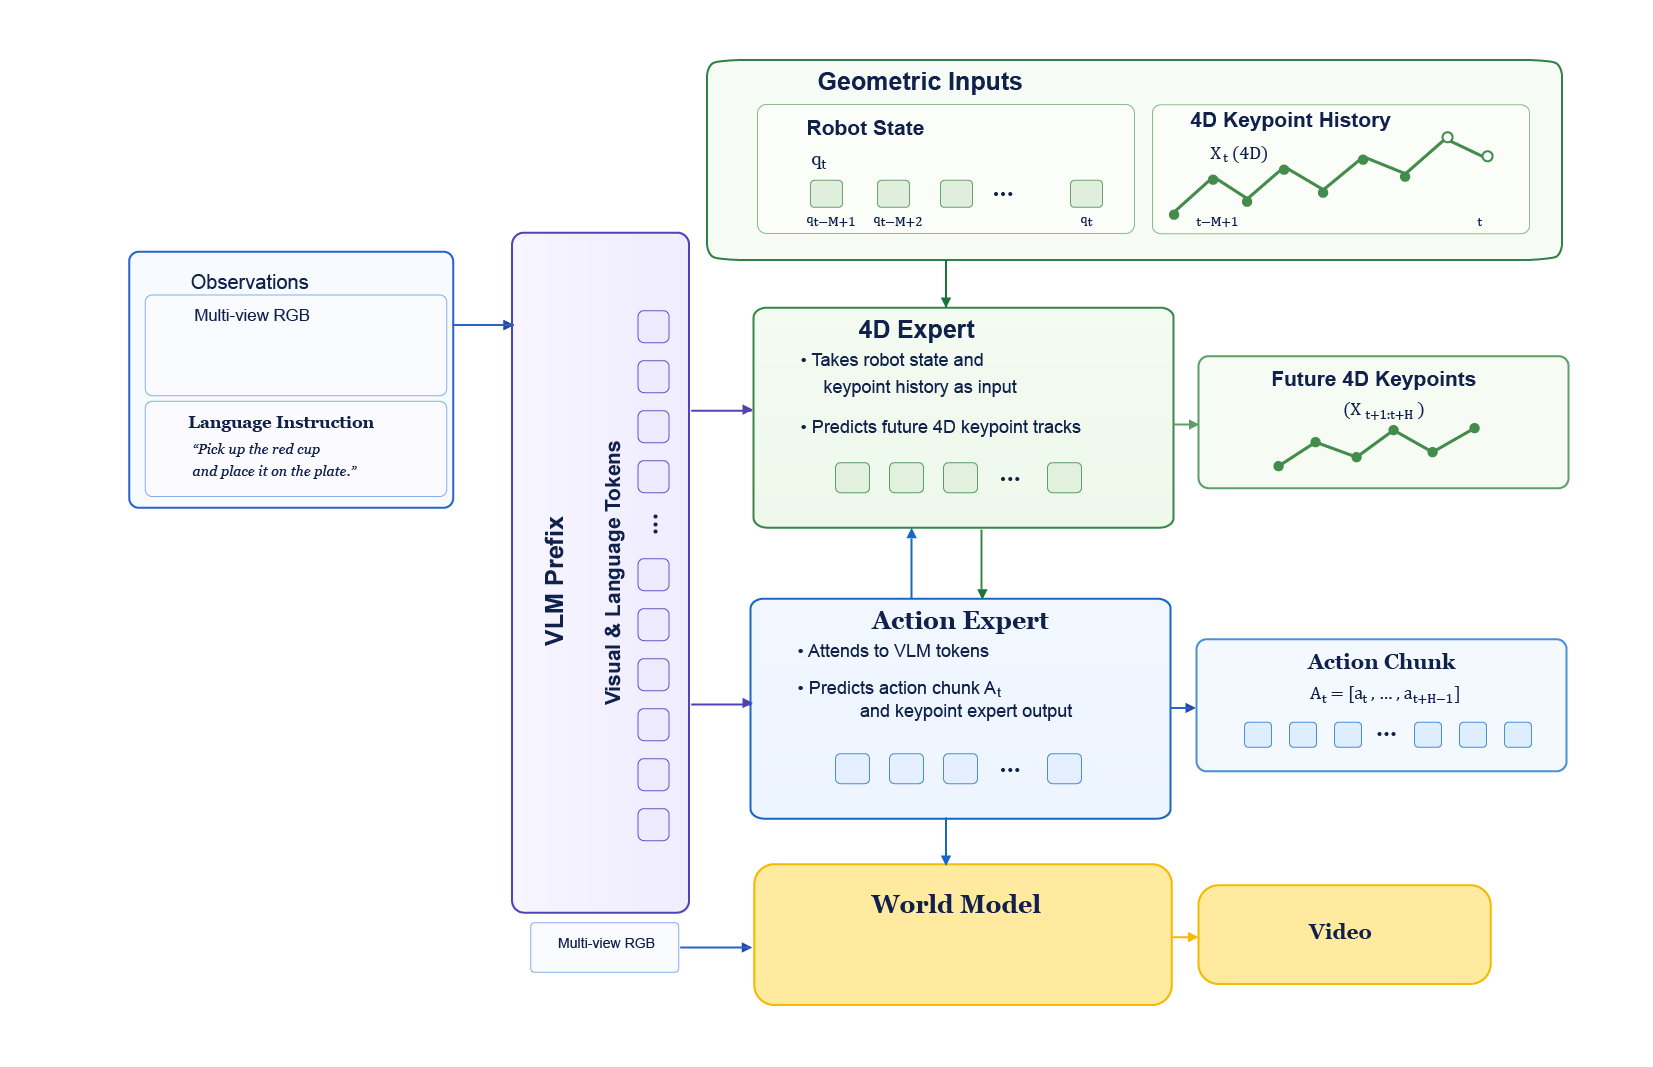
\includegraphics[width=\textwidth]{TrajMoT_VLA_Figure1_Vector_1_2.png}
    \caption{\textbf{4DW-VLA architecture.}
    A frozen VLM prefix encodes multi-view RGB and the language instruction.
    A dedicated \textbf{4D keypoint expert} takes robot state $q_t$ and a
    history of FK-derived 4D keypoint tracks $X_t$ as input and predicts
    future 4D keypoint tracks $X_{t+1:t+H}$; the \textbf{action expert}
    attends to the VLM prefix and to the 4D keypoint expert's output to
    predict the action chunk $A_t$. A frozen video world model, conditioned
    on the same multi-view RGB, supervises the shared representation during
    training only. At deployment the world model is dropped, but the 4D
    keypoint expert is retained and continues to condition the action
    expert on metric 4D structure.}
    \label{fig:overview}
\end{figure*}

\subsection{Problem Formulation}

We consider language-conditioned visuomotor control as modeling
\begin{equation}
p\bigl(A_t \mid o_t, \ell_t, q_t\bigr),
\label{eq:policy}
\end{equation}
where $o_t$ denotes multi-view RGB observations (head and wrist cameras),
$\ell_t$ is the language instruction, $q_t$ is proprioception, and
$A_t = [a_t, a_{t+1}, \ldots, a_{t+H-1}]$ is an action chunk of horizon~$H$.
We train a conditional generative action expert (flow matching or diffusion)
to approximate this distribution, while an auxiliary keypoint expert predicts
4D tracks and a set of learnable foresight tokens, carried inside the action
expert's own suffix stream, are distilled against a frozen video foundation
model over a compatible horizon~$T$.

\subsection{Embodiment-Centric 4D Keypoint Trajectories}

Robots already expose the quantities needed for metric 4D supervision. For
each keypoint $k \in \{1,\ldots,K\}$ on the kinematic chain (major arm joints
and both end-effectors),
\begin{equation}
p^k_t = \mathrm{FK}_k(q_t) \in \mathbb{R}^3
\label{eq:fk}
\end{equation}
is the Cartesian position in the robot base frame.
Stacking keypoints over a short history window
yields a history tensor $P^{\mathrm{hist}}_t$, which the keypoint expert
attends to together with the frozen VLM prefix (Section~\ref{sec:fusion}) to
produce a per-timestep query representation. That representation is
projected through a shared output head to obtain two predictions: the
current-frame keypoints $\hat{p}^k_t$, used as a reconstruction target, and
the future keypoints $\hat{p}^k_{t+1:t+H}$ over the action horizon~$H$,
obtained by adding a learned per-step future positional embedding to the
same query before reprojection, so the future and current predictions
share weights rather than coming from two separate sub-networks. Supervision
combines a current-frame term and a future-trajectory term,
\begin{equation}
\mathcal{L}_{\mathrm{kpt}} = \beta \Bigl(
    \operatorname{MSE}\bigl(\hat{p}_t, p_t\bigr)
    + \gamma\, \operatorname{MSE}\bigl(\hat{p}_{t+1:t+H}, p_{t+1:t+H}\bigr)
\Bigr),
\label{eq:loss4d}
\end{equation}
where each $\operatorname{MSE}(\cdot,\cdot)$ averages squared error over the
$K$ keypoints and their 3 coordinates (and, for the future term, over the
horizon~$H$ as well), $\beta$ is the overall keypoint-loss weight, and
$\gamma$ weights the future term relative to the current-frame term.
Ground-truth keypoints are computed from recorded $q_{t+\tau}$ via the same
FK, so no external point tracker or scene reconstruction is required. This
is the same privileged-body idea as ELAN4D~\cite{elan4d2026}, lifted from an
auxiliary residual branch into a \textbf{first-class input-and-output} of a
WAM.

\subsection{Distilled Visual Foresight from Observation, Instruction, and
State}

Rather than a separate head with its own encoder, foresight is carried by
$M$ \textbf{learnable foresight tokens} $Z^{\mathrm{fs}}_t \in
\mathbb{R}^{M \times d}$, appended to the action expert's own suffix stream
alongside the action tokens. Because the action expert attends to the
prefix, the keypoint expert, and its own suffix (Section~\ref{sec:fusion}),
$Z^{\mathrm{fs}}_t$ is conditioned on the predicted future keypoints
$\hat{p}_{t+1:t+H}$ through that shared attention path, without a
dedicated video-to-4D cross-attention edge. Supervision is a genuine
flow-matching objective against a \textbf{frozen} video diffusion
transformer (DiT) $g_{\mathrm{wan}}$ (WAN2.2-TI2V-5B): the real future frames
$o_{t+1:t+T}$ are encoded by the frozen WAN2.2 VAE into a latent $x_0$,
corrupted along a linear path $x_\tau = (1-\tau) x_0 + \tau \epsilon$ with
$\epsilon \sim \mathcal{N}(0, I)$ and $\tau \sim U[0,1]$, and $g_{\mathrm{wan}}$
is trained to predict the corresponding denoising velocity $\epsilon - x_0$,
conditioned on $x_\tau$ and on the projected foresight tokens
$h(Z^{\mathrm{fs}}_t)$ supplied as cross-attention context. This is
structurally identical to the action expert's own flow-matching loss on
action chunks, except that $g_{\mathrm{wan}}$'s weights are frozen
throughout and only $h$ and the upstream foresight tokens are
updated.\footnote{This is a genuine generative-modeling objective evaluated
at training time rather than a feature-distillation loss: the target is a
real noised video latent, and $g_{\mathrm{wan}}$ performs the same one-step
velocity prediction it performs during iterative sampling, so no frames are
actually generated during training. This video/flow-matching mechanism follows
prior work~\cite{internvla15}; 4DW-VLA's contribution is routing the
foresight tokens through the same keypoint-expert-aware attention paths as
the action expert, not a new video objective.}

\subsection{Heterogeneous Multimodal Fusion}
\label{sec:fusion}

The design in Fig.~\ref{fig:overview} is motivated by the three pain
points in Section~\ref{sec:intro}, not by a single fusion block:
\begin{itemize}
\item \textbf{Modalities.} Images, video, text, 3D/4D geometry, and (in the
  broader framework) tactile and force streams. The current RoboTwin
  instantiation uses RGB, language, proprioception, and FK 4D; force~/~tactile
  remain architectural slots (Section~\ref{sec:limitations}).
\item \textbf{Who attends to whom.} Text attends to images (VLM
  cross-attention). The keypoint expert attends to the prefix and to
  history 4D tracks. The action expert attends to \textbf{all} three streams
  (prefix, keypoint expert, and its own suffix, which also carries the
  distilled foresight tokens), because control must bind semantics,
  geometry, and dynamics. Fig.~\ref{fig:mask} shows the resulting
  block-causal attention mask directly.
\item \textbf{Early~/~late~/~full fusion.} Proprioception and 4D tracks,
  being low-dimensional and metric, are fused late with VLM tokens; RGB and
  language are fused early inside the frozen VLM.
\item \textbf{Rates.} Cameras are modeled at 25\,Hz; force-control loops
  (when present) at 100\,Hz. Rate-aware sampling avoids naively duplicating
  high-rate tokens in the VLM context.
\end{itemize}

\begin{figure}[t]
    \centering
    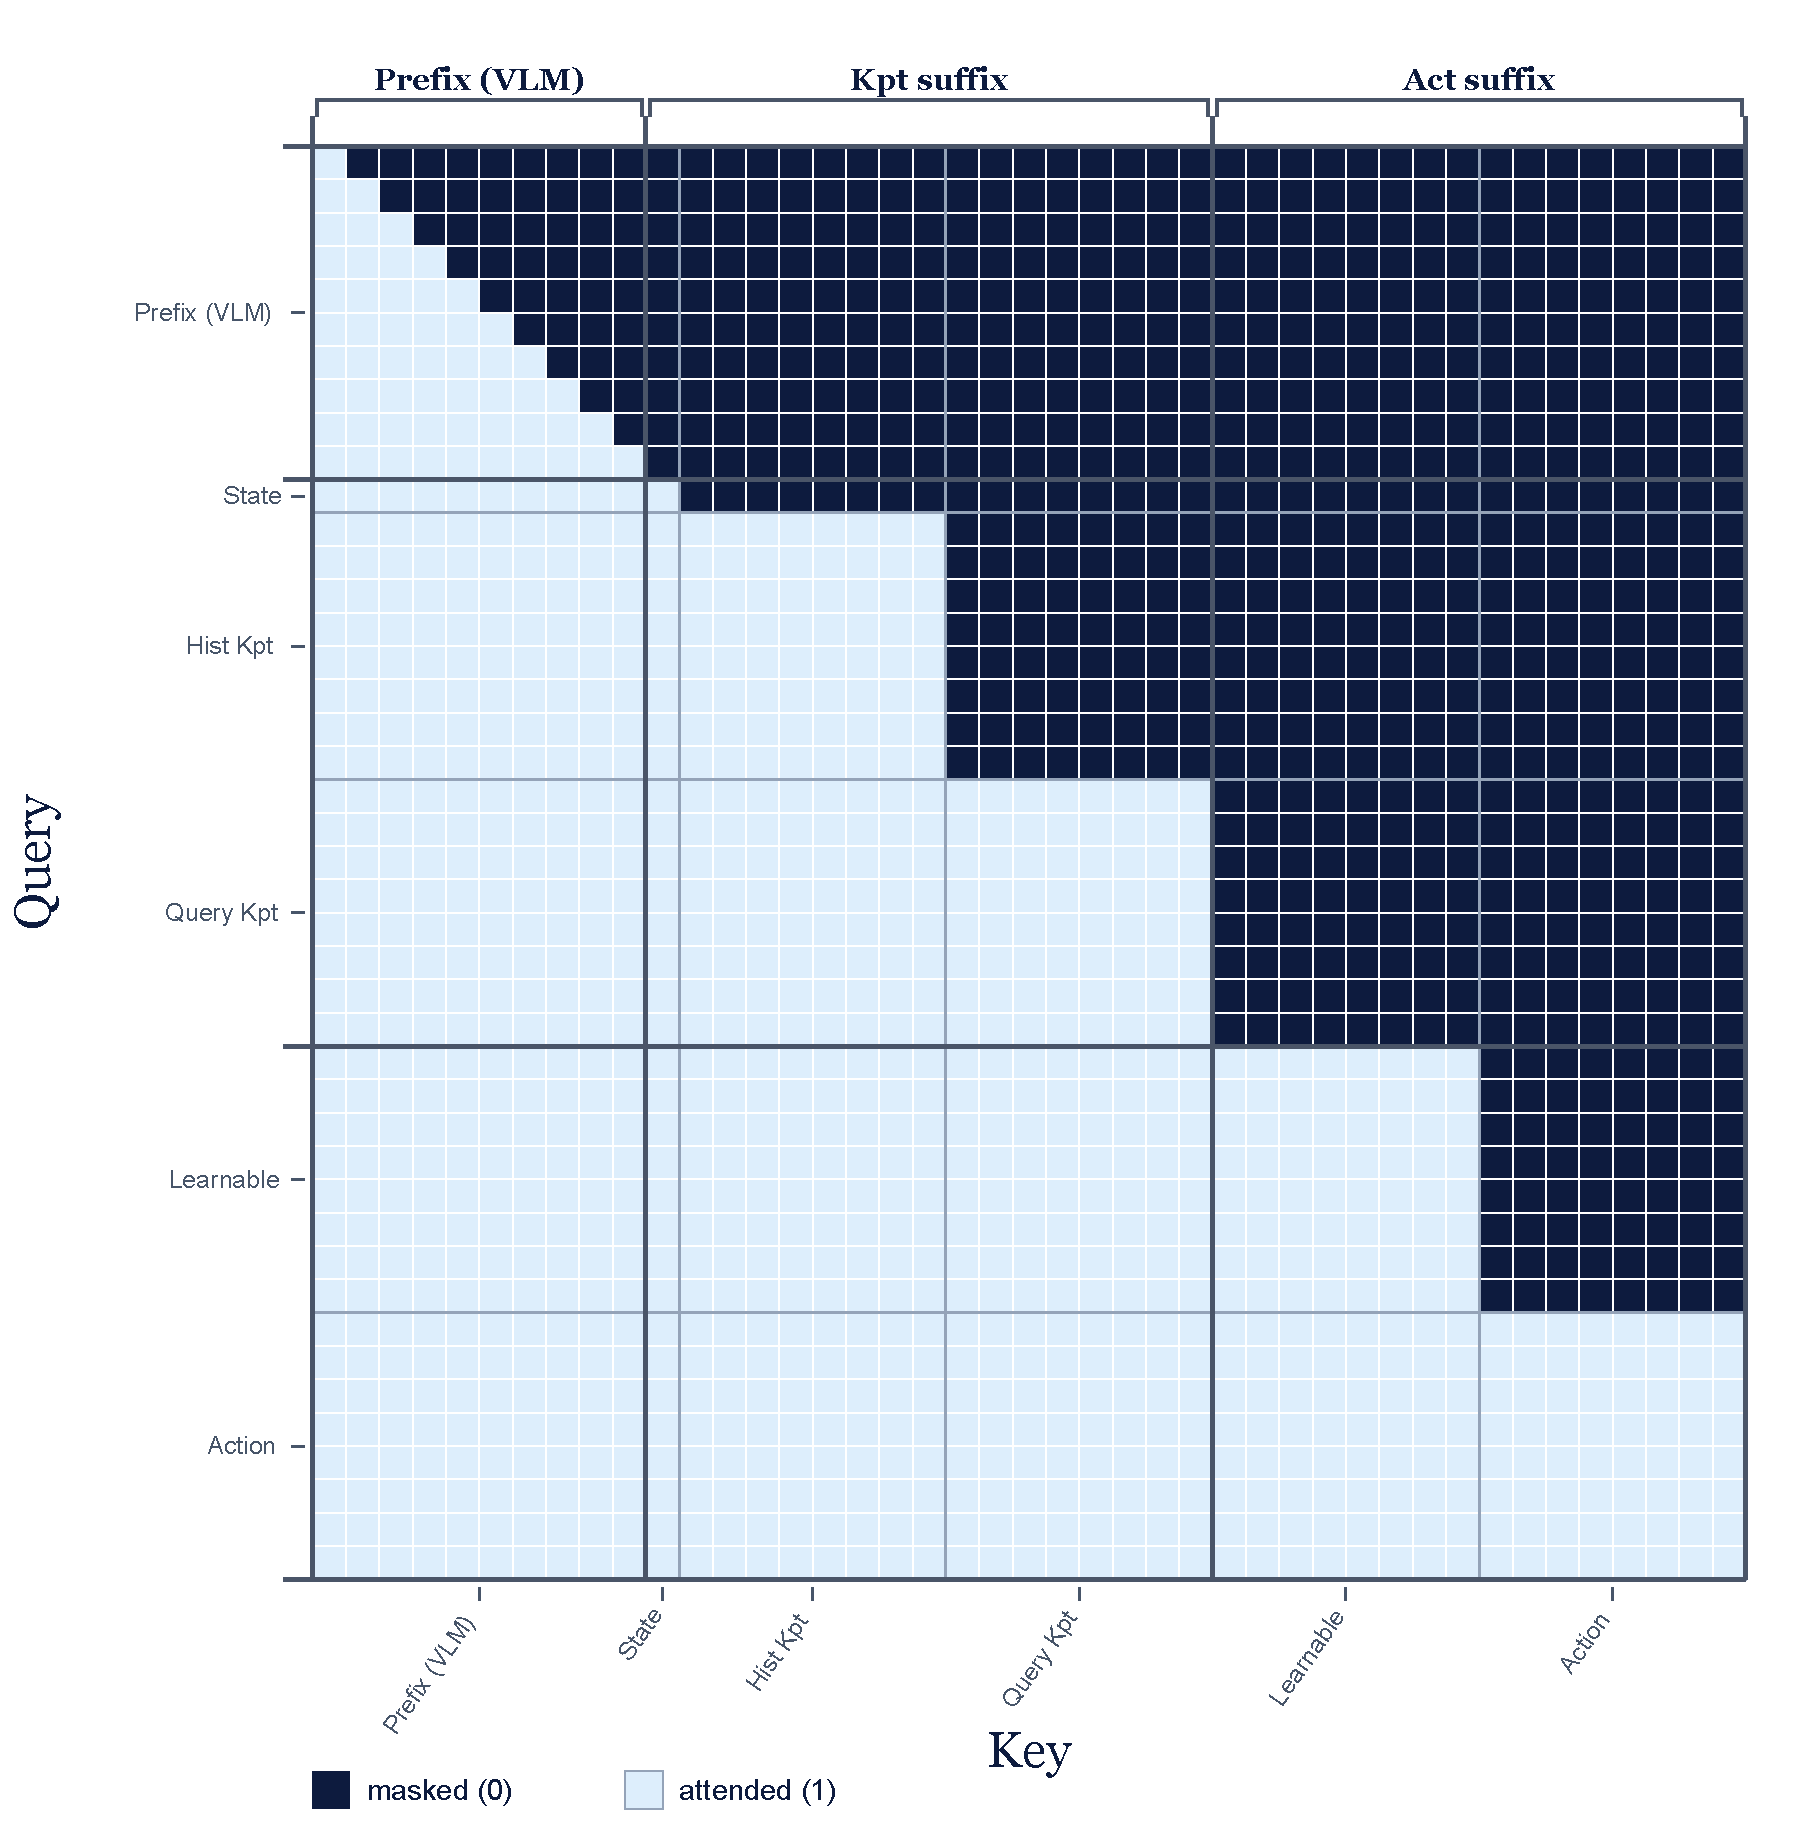
\includegraphics[width=\linewidth]{TrajWM-VLA_mask.pdf}
    \caption{\textbf{Block-causal attention mask.} Rows are query blocks,
    columns are key blocks; light cells are attended, dark cells are
    masked. The VLM prefix attends causally only to itself. The keypoint
    expert (proprioceptive state, history keypoints, and future-keypoint
    queries) attends to the prefix and to itself. The action expert
    (learnable foresight tokens and action queries) attends to the
    prefix, the keypoint expert, and itself, the only block with access to
    all three streams.}
    \label{fig:mask}
\end{figure}

These choices are a \emph{design language} for later sensors, not a claim
that every slot is active in the experiments of Section~\ref{sec:experiments}.

\subsection{Multi-Task Objective and Staged Warmup}

Training minimizes a stationary multi-task loss
\begin{equation}
\mathcal{L} = \lambda_{\mathrm{act}}\mathcal{L}_{\mathrm{act}}
    + \lambda_{\mathrm{vqa}}\mathcal{L}_{\mathrm{vqa}}
    + \lambda_{\mathrm{vid}}\mathcal{L}_{\mathrm{vid}}
    + \mathcal{L}_{\mathrm{kpt}}.
\label{eq:loss}
\end{equation}
$\mathcal{L}_{\mathrm{act}}$ is the action-expert denoising~/~flow-matching
loss on expert chunks, and $\mathcal{L}_{\mathrm{vqa}}$ is a next-token
cross-entropy loss that keeps the underlying VLM's VQA and sub-task
prediction capability (Section~\ref{sec:related}) intact during
post-training. $\mathcal{L}_{\mathrm{kpt}}$ already carries its own internal
weights $\beta$ and $\gamma$ (Eq.~\ref{eq:loss4d}), so it enters the total
loss without an additional coefficient. The remaining coefficients
$\lambda_{\cdot}$ are fixed hyperparameters.

\textbf{Staged post-training.}
\begin{enumerate}
\item \textbf{Warmup (400 steps).} Update the keypoint expert and the
  foresight-distillation projection at the default rate; keep the VLM
  frozen; scale the action expert's learning rate down to $0.04\times$ the
  default rate. This lets the newly-initialized keypoint expert and
  foresight tokens learn quickly while limiting how much the
  already-pretrained action expert drifts during the short warmup.
\item \textbf{Joint post-training (76 epochs).} Continue with the VLM frozen.
  The three compared methods use the same 76-epoch post-training schedule.
\end{enumerate}

\subsection{Inference: Action Prediction Only}

At deployment we simply evaluate the trained
policy $\pi_\theta$ on the current observation, instruction, and
proprioception to obtain the action chunk $A_t$.
Unlike prior work~\cite{nvidia2026wam,internvla15}, where the entire auxiliary path is
discarded at inference, the keypoint expert is \textbf{retained}: it
continues to attend to the frozen VLM prefix and to history 4D tracks
$P^{\mathrm{hist}}_t$ (computed from $q_t$ via FK, not from an external
sensor), and the action expert continues to attend to it, so 4D
conditioning persists into deployment. Only the video-generation branch is
dropped: the learnable foresight tokens are still produced inside the
action expert's own suffix, but the frozen video DiT $g_{\mathrm{wan}}$
that would consume them for generation is neither invoked nor loaded at
deployment (Section~\ref{sec:method}), so no video-generation cost is
paid. The deployed policy therefore keeps the keypoint expert's extra
forward pass and its FK-derived input; only the future-video head matches
the ``train with foresight, drop at test time'' pattern.

% ====================================================================
\section{Experiments}
\label{sec:experiments}

We evaluate 4DW-VLA on RoboTwin~2.0~\cite{chen2025robotwin2} and compare
against recent foundation VLAs. We aim to answer:
\begin{enumerate}
\item Does co-training the 4D keypoint expert with distilled visual
  foresight improve in-domain (Easy) success over strong VLA baselines
  under a common 76-epoch post-training budget?
\item Does the same recipe improve robustness on the Hard
  (domain-randomized, OOD) split?
\item Does the trend persist across stacking, tool-use scanning, and
  placement tasks?
\end{enumerate}

\subsection{Experimental Setup}

\textbf{Benchmark.}
RoboTwin~2.0 is a dual-arm manipulation suite on SAPIEN with strong domain
randomization along clutter, lighting, background texture, table height, and
language~\cite{chen2025robotwin2}. We follow the public Easy~/~Hard protocol:
Easy corresponds to \texttt{demo\_clean}; Hard to
\texttt{demo\_randomized}. Evaluations use the Aloha-AgileX bimanual
embodiment. Success rate is the metric.

\textbf{Tasks.}
\begin{itemize}
\item \texttt{stack\_bowls\_three}: stack three bowls. The task is
  geometrically precise and contact-rich.
\item \texttt{scan\_object}: one arm grasps a scanner, the other grasps an
  object, then the scanner is used on the object. This stresses dual-arm
  coordination and tool use.
\item \texttt{place\_bread\_skillet}: place bread in a skillet. This provides
  an additional placement task for testing robustness across a different
  manipulation objective.
\end{itemize}

\textbf{Baselines.}
InternVLA-A1.5~\cite{internvla15} (Shanghai AI Laboratory) unifies
understanding, latent foresight, and action;
LingBot-VLA~2.0~\cite{lingbot2026} (Robbyant~/~Ant Group) is a 6B
cross-embodiment VLA with predictive-dynamics distillation. InternVLA-A1.5
and 4DW-VLA are both trained and evaluated in our own codebase under a
common \textbf{76-epoch} post-training schedule; 4DW-VLA additionally
uses the 400-step keypoint-and-foresight warmup, a frozen VLM, and a
$0.04\times$ action-expert learning-rate scale during warmup
(Table~\ref{tab:recipe}).
\textbf{LingBot-VLA~2.0 is not reproduced by us}: we do not have its
checkpoint, training code, or configuration, so its numbers are taken
as-reported from its own release and are not independently verified to
have used a matching schedule. The schedule-matching claim above therefore
applies only to InternVLA-A1.5 and 4DW-VLA; LingBot-VLA~2.0 should be
read as an external reference point, not a controlled comparison.
LingBot-VLA~2.0 was not evaluated on \texttt{scan\_object} or
\texttt{place\_bread\_skillet} (denoted n/a).

\begin{table*}[t]
\centering
\caption{\textbf{Post-training success rates (\%) on RoboTwin~2.0.}
Easy = \texttt{demo\_clean}; Hard = \texttt{demo\_randomized} (OOD).
Bold is best in each column. LingBot-VLA~2.0 was not evaluated on
\texttt{scan\_object} or \texttt{place\_bread\_skillet}.}
\label{tab:main}
\small
\setlength{\tabcolsep}{4pt}
\begin{tabularx}{\textwidth}{lCCCCCC}
\toprule[1.5pt]
 & \multicolumn{2}{c}{\texttt{stack\_bowls\_three}}
 & \multicolumn{2}{c}{\texttt{scan\_object}}
 & \multicolumn{2}{c}{\texttt{place\_bread\_skillet}} \\
\cmidrule(lr){2-3} \cmidrule(lr){4-5} \cmidrule(lr){6-7}
Method & Easy & Hard & Easy & Hard & Easy & Hard \\
\midrule
InternVLA-A1.5          & 71 & 56 & \textbf{45} & 28 & 31 & 20 \\
LingBot-VLA~2.0         & 78 & 22 & n/a & n/a & n/a & n/a \\
\textbf{4DW-VLA (ours)} & \textbf{81} & \textbf{58} & \textbf{45}
                          & \textbf{33} & \textbf{39} & \textbf{29} \\
\bottomrule[1.5pt]
\end{tabularx}
\end{table*}

\begin{table}[t]
\centering
\caption{\textbf{4DW-VLA post-training recipe.}}
\label{tab:recipe}
\small
\begin{tabularx}{\linewidth}{@{}lX@{}}
\toprule[1.5pt]
Item & Setting \\
\midrule
Benchmark & RoboTwin 2.0 \\
Post-training budget & 76 epochs (all methods) \\
Warmup & 400 steps on keypoint + foresight heads \\
VLM & Frozen \\
Warmup LR scale (action) & $0.04\times$ default \\
Easy~/~Hard & \texttt{demo\_clean}~/~\texttt{demo\_randomized} \\
\bottomrule[1.5pt]
\end{tabularx}
\end{table}

\subsection{Main Results}

Fig.~\ref{fig:results} visualizes Table~\ref{tab:main}.

\begin{figure*}[t]
    \centering
    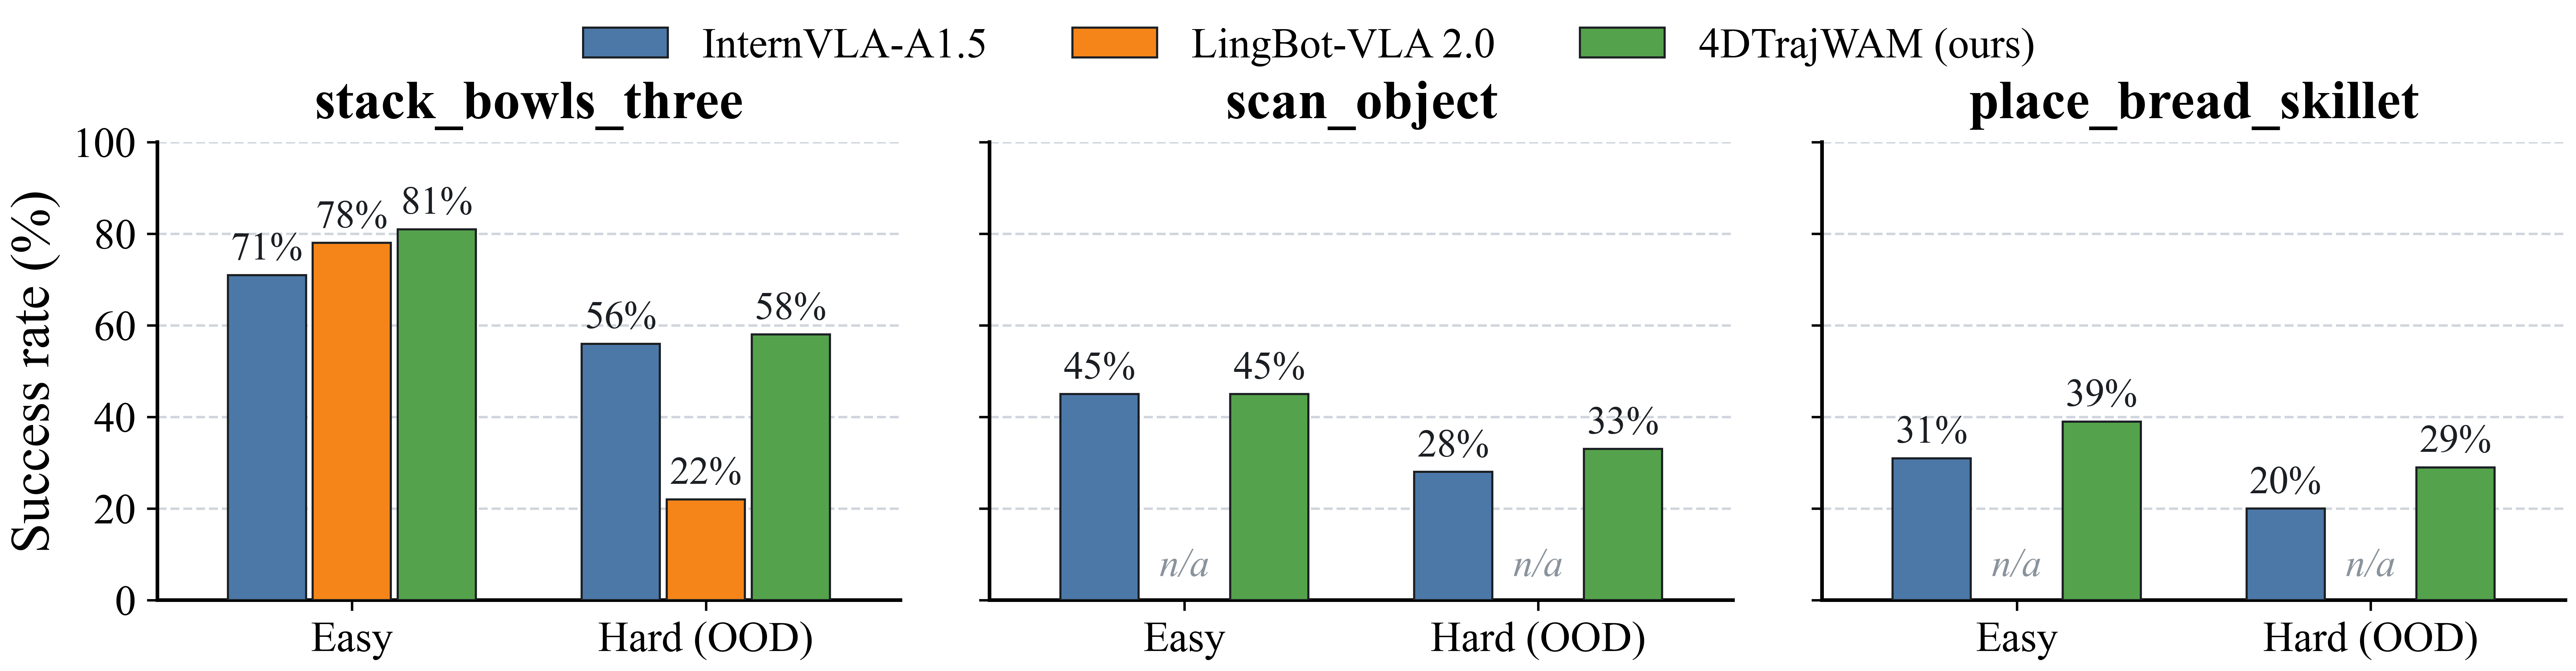
\includegraphics[width=\textwidth]{fig5_results.png}
    \caption{\textbf{RoboTwin~2.0 success rates.} Grouped bars for Easy and
    Hard (OOD) on three tasks. LingBot-VLA~2.0 is not evaluated on
    \texttt{scan\_object} or \texttt{place\_bread\_skillet} (n/a). All three
    methods use the reported 76-epoch post-training schedule.}
    \label{fig:results}
\end{figure*}

\textbf{\texttt{stack\_bowls\_three}.}
4DW-VLA attains 81\% Easy and 58\% Hard, exceeding InternVLA-A1.5
(71\%~/~56\%) and LingBot-VLA~2.0 (78\%~/~22\%). The Easy ranking is tight
(81 vs.\ 78 vs.\ 71), as expected when all methods are evaluated after the
same reported schedule. The Hard split is not: LingBot-VLA~2.0 drops to 22\%,
while 4DW-VLA remains slightly above InternVLA-A1.5 (58\% vs.\ 56\%). We
interpret this result as consistent with the hypothesis that metric FK tracks
complement visual dynamics priors in randomized scenes, rather than as proof
of a single-module causal effect.

\textbf{\texttt{scan\_object}.}
InternVLA-A1.5 and 4DW-VLA both reach 45\% Easy. On Hard, 4DW-VLA
reaches 33\% versus 28\%. The improvement is modest but suggests that the 4D
body trajectory gives the action expert a more stable geometric reference for
dual-arm tool use when visual context is randomized.

\textbf{\texttt{place\_bread\_skillet}.}
4DW-VLA reaches 39\% Easy and 29\% Hard, compared with 31\% and 20\% for
InternVLA-A1.5. The absolute gains are 8 and 9 percentage points,
respectively. Since LingBot-VLA~2.0 has no result for this task, this
comparison is limited to InternVLA-A1.5.

Across the three tasks, 4DW-VLA is the best reported method in every
evaluated column. Relative to InternVLA-A1.5, the absolute Hard improvements
are +2 points on \texttt{stack\_bowls\_three}, +5 points on
\texttt{scan\_object}, and +9 points on \texttt{place\_bread\_skillet}.
Relative to LingBot-VLA~2.0, the Hard improvement on
\texttt{stack\_bowls\_three} is +36 points. Confidence intervals are not yet reported
(Section~\ref{sec:limitations}).

\subsection{What the Numbers Do and Do Not Show}

The Easy score improves over InternVLA-A1.5 on both
\texttt{stack\_bowls\_three} and \texttt{place\_bread\_skillet}, and matches
it on \texttt{scan\_object}, indicating that the predictive auxiliary heads
do not hurt in-domain post-training under the frozen-VLM recipe. The
consistent Hard gains over InternVLA-A1.5 are compatible with the proposed
4D spatial prior.

These results cannot yet isolate 4D prediction from foresight-distillation
co-training or the warmup schedule, nor establish whether the remaining gap
to InternVLA-A1.5 is caused by architecture, optimization details, data
order, or random seeds. The comparison should therefore be read as evidence
supporting the design hypothesis, not as a complete ablation study.

\subsection{Real-Robot Validation (In Progress)}
\label{sec:realrobot}



\begin{table}[t]
\centering
\caption{\textbf{Real-robot validation protocol (results pending).}}
\label{tab:realrobot}
\small
\begin{tabularx}{\linewidth}{@{}lX@{}}
\toprule[1.5pt]
Item & Setting \\
\midrule
Platform & TBD \\
Tasks & TBD subset of the three RoboTwin~2.0 tasks above \\
Trials per task & TBD \\
Compared methods & 4DW-VLA vs.\ InternVLA-A1.5 \\
Metric & Success rate \\
\bottomrule[1.5pt]
\end{tabularx}
\end{table}

% ====================================================================
\section{Limitations}
\label{sec:limitations}

This work has several limitations.
\begin{itemize}
\item \textbf{Limited task set.} Three RoboTwin~2.0 tasks are reported, while
  average performance over the full benchmark is unknown.
\item \textbf{The fusion-mechanism claim needs a direct ablation.} We argue
  that a dedicated, retained-at-deployment 4D keypoint expert is preferable
  to token-concatenation (GeoPredict-style) or a residual decoder discarded
  at inference (ELAN4D-style), but Table~\ref{tab:main} only shows that
  the three-path design with a keypoint expert outperforms baselines; it
  does not yet compare fusion mechanisms directly, nor test whether performance
  would drop if the keypoint expert were dropped at inference instead of
  retained. Both ablations are needed before the fusion-mechanism claim can
  be reported as demonstrated rather than argued. We also cannot yet
  separate the 4D-prediction and foresight-distillation objectives, or the
  warmup length and the $0.04\times$ action-expert learning-rate scaling,
  from each other.
\item \textbf{Incomplete evaluation metadata.} Trial counts, random seeds,
  and confidence intervals for each baseline are not yet fully reported.
\item \textbf{Uninstantiated framework slots.} Tactile~/~force streams,
  100\,Hz control, reinforcement or evolutionary fine-tuning, and contrastive
  alignment are design goals, not measured components.
\item \textbf{Simulation only.} All numbers in Table~\ref{tab:main} are
  from simulation. Sim-to-real transfer of FK-derived 4D keypoints is
  expected to be straightforward, but vision-side WAM transfer is untested.
\item \textbf{Incomplete implementation details.} Loss coefficients, $K$,
  $H$, $T$, video-backbone specifics, and action-expert internals are not
  yet fully specified.
\end{itemize}

% ====================================================================
\section{Conclusion}
\label{sec:conclusion}

We presented 4DW-VLA, a three-path mixture-of-transformers that gives
embodiment-centric 4D keypoint trajectories a dedicated expert retained at
deployment, co-trained with a distilled visual-foresight head that is
dropped at inference. On three RoboTwin~2.0 tasks, 4DW-VLA matches or
exceeds two recent VLA baselines across all splits, with the largest gains
under domain randomization. Future work includes direct ablation of the
fusion mechanism (token-concatenation and residual-decoder baselines),
instantiation of the force and tactile slots, evaluation on the full
benchmark, and real-robot validation on a bimanual platform.

% ====================================================================
\bibliographystyle{plainnat}
\bibliography{references}

\end{document}
